% ------------------------------------------------------------------------ %
% !TEX encoding = UTF-8 Unicode
% !TEX TS-program = pdflatex
% !TEX root = ../Tesi.tex
% !TeX spellcheck = en_US
% ------------------------------------------------------------------------ %
%
% ------------------------------------------------------------------------ %
% 	Problem analysis and proposed solution
% ------------------------------------------------------------------------ %
%
\chapter{Problem Analysis}
%
\label{cap:probanalysis}
%
% ------------------------------------------------------------------------ %
%

In this chapter the specific problems of this work will be detailed and analyzed, explaining what are the limits and the constraints the challenge has. The chapter starts with a brief recap, followed by the proper definition of what I faced, while in the last part there is a list of constraints my architecture will have fulfilled in order to have a universal and functional solution.
  

\section{Contextualization} \label{facedProblem}
As already explained introducing this thesis work in \ref{motivation}, I studied in deep the Android operating system to find, and later implement a concrete solution, to the problem I will define and describe in dept in this section. All the work done by me is focused on Android because every mobile operating system is different to each other and has proprietary working mechanism which have to be studied separately. Since there are many more Android devices than any other mobile OS, and Android is an open source software and there is no need to buy development licenses or proprietary hardware or software like using for example Apple systems, I decided to work with it, even if by studying another mobile OS and implementing the same concepts of my solution it is certainly possible to achieve the same result i got by working only with Android. 
In the previous chapter, number \ref{cap:statoarte}, I have defined Android OS working mechanism and components, pointing out the main focus on intent generation and resolution mechanism. I have then defined in deep what a distributed system is and should be, explaining connection mechanism architectures and properties.\\ 
The Android OS is a centralized operating system designed for a single physical user, to be used on personal mobile devices such as smartphones and tablets. The result of this Google's ideas is that in contemporary society there is a wide spread of Android devices, which now have computing capacity comparable to normal desktops and notebooks. Many people have multiple devices which they use separately: typically they use smartphones for calls and  work emails and maybe tablets to easily surf the Internet and play games, but what they can not do is use them together to perform a common task easily. Android, in fact, has not been thought to build a real distributed system, the networking functionalities are designed to exchange messages, and to replace standard personal computers in some task as indeed sending emails.
The result is a non collaborative confused cloud of devices, which are connected to the net, but are not really connected themselves to cooperate. Solutions are often partial or proprietary and closed, even if some useful solutions exist.\\
The idea is let android devices collaborate and cooperate in a \textit{Liquid environment} like the one presented in section \ref{liquid computing}. The fundamental requirement is the implementation of an android service, able to build and maintain a distributed net of android devices over a Wi-Fi LAN (Local Area Network), and then let one, or more devices in that net generate Android intents and distribute them one, or more, of the other devices involved. Thus in this chapter I am considering only Android devices that can be connected in a WiFi LAN.\\
After this brief recap of what has been said about the Android OS and distributed systems in the state of the art chapter, here I am trying to define with more precision the problem I am going to face: which its constraints and its possible goals are.

\section{Considered Devices}
As anticipated above, I am going to take into account only devices that can be somehow connected to a LAN, but as described in \ref{connectivity} Android devices are built to be connected to the Internet and most of them comes with a WiFi chip integrated. Another \textit{"little relaxation"} I want to do is linked to the variety of Android OS versions. I want to take into account only devices updated to at least version 4.4 (API level 19). This is due to the fact that starting from Android KitKat (4.4 version) Google brought some important improvements  to the libraries of the framework and in addition, according to the \tablename~\ref{tab:chart}, with this choice it is possible to cover the 84\% of the active Android devices.\\
Having done these clarifications, now I am defining the problem.

\section{Definition} \label{problemdefinition}
\textit{How can we transform a standard mobile OS into a distributed version of it?} This is the general question I want to give an answer in this work.
As already said the Android OS is a pretty closed system itself, the intent resolution mechanism shows how it is difficult to let communicate various components inside a single device. On the other hand it is equally true that Android devices are real powerful modern computers and would be great if somehow it could be possible to have a device able to detect other devices in a LAN send data and task to perform in a transparent way and then get back, if necessary, result or data. Let me be more concrete, often in a home environment there are several android devices, with a distributed intent resolution mechanism it would be possible for example to take a photo from one device with the camera of another one, to generate an intent to open a file on a group of devices simultaneously, to play a video remotely and so on, only by generating intents and then send them to the distributed net. \textit{How can we let multiple android devices act as a single big distributed system?} This is the question that my thesis is trying to answer. My work is a concrete solution, it is about defining and creating a method to distribute android intents from one device to other in a LAN and then let the OS act as usual to manage and resolve them.\\
So I am trying to let different android devices talk by means of distributing intents using  well known architecture: a master component, let me call it \textit{distributed intent generator} acting as client, and a slave component \textit{distributed intent solver} acting as a server. The two components i will realize will be common Android background services registered on the WiFi LAN. Both of these components will result in android applications so that a single device could be used to control others or to be controlled.\\
In \figurename~\ref{fig:3.1} is presented how such a system should work once the net is up. The distributed system in figure is a simplification of what the middleware for distributing intents will do. The architecture will communicate using standard android networking messages that are build on top standard protocols of the ISO/OSI stack.
 
\begin{figure}[h]
	\centering
	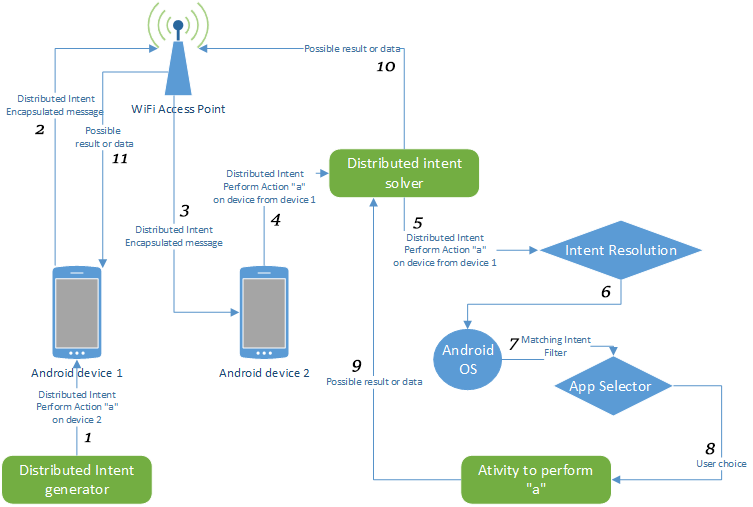
\includegraphics[width=.95\textwidth]{scheme}
	\caption{Distributed intent resolution}
	\label{fig:3.1}
\end{figure}

The important point is having a message with a well defined content: it is what the two parts must write and read, so it has to be clear for machines, must be compliant with all the requests of \textit{M2M (Machine-to-Machine) communication}. This type of communications is a constraint of my work and are explained in the next section \ref{problemconstraints}.Another important point is let the Android OS work as it is designed for, the main aim of this thesis work is to build a middleware to let distribute native Android intents over the network. This is a new approach to this problem in fact, there are yet some android applications which let the user send stream or data to other devices in a LAN but, with specialized and ad hoc built messages within the same application context, using a mechanism really close to explicit intent resolution. My middleware is supposed to address the problem using a more general approach and a mechanism equal to implicit intent resolution. What I'm doing is create a system to spread any kind of implicit intent and let the OS react as usual to perform the required action.
It is not even marginal the choice of the type of network to be used in such a system. Android devices are in fact, usually, mobile devices, and for this reason they can be easily moved from one place to another, so the network must take into account this property dynamically react to continuous changes.\\
Next sections will properly define all the constraints of the given problem and propose a solution that fulfills them all.
\section{Probelm scenarios}
As already anticipated with the definition of the problem,  the aim of this thesis is to give the feeling, to users, that they are working with multiple Android devices as if they were one single distributed operating system. I want to analyze some problematic scenarios an then in the next chapter of the thesis provide, if possible a solution to each specific case.

\subsubsection{Background working middleware}
 \begin{figure}[h]
	\centering
	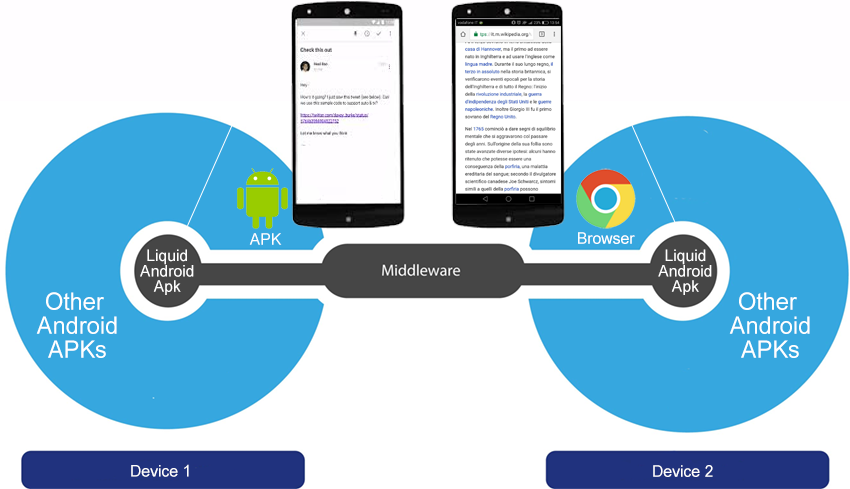
\includegraphics[width=.85\textwidth]{esempio1}
	\caption{Liquid Android working example}
	\label{fig:3.3}
\end{figure}
\begin{figure}[h]
	\centering
	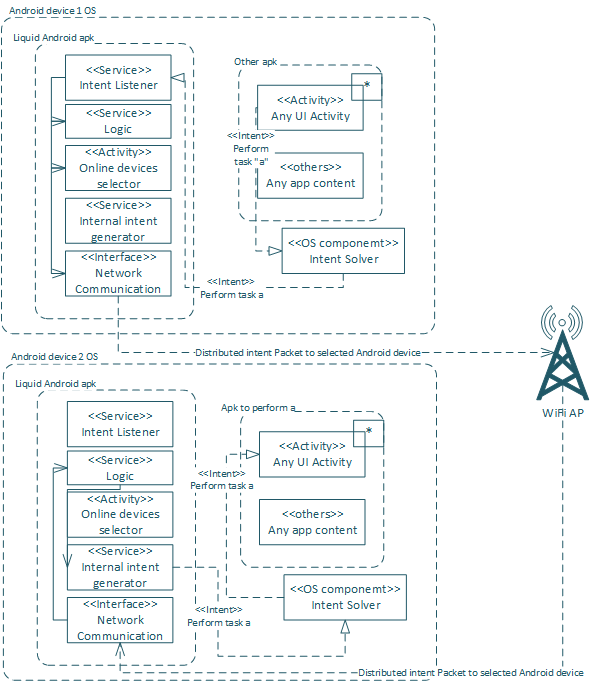
\includegraphics[width=.85\textwidth]{scenario1}
	\caption{Liquid Android working as stand alone middleware APK}
	\label{fig:3.2}
\end{figure}
 

In the best case, the result to be achieved would be a single Android APK, to be installed on devices as background bunch of services acting as a middleware. Liquid Android services which providing a communication interface can listen distributed events invocations and react to them automatically. The middleware may intercept local intents, find online devices in the distributed network, let the user select on which of them execute the task and send the intent to the selected remote Android device.\\
The \figurename~\ref{fig:3.2} shows a possible UML component diagram of the Liquid Android middleware, the scheme points out the interactions between the Liquid Android application (APK) and other possible applications installed on the device. The group of services intercepts the local intent, created by a different application in the same device, let the user of the system select on which available device execute the task, build and spread the the distributed intent message on the LAN, and when the message arrives at the other device the middleware transform the received message in a local intent to be resolved as usual by the operating system.\\
I want to provide a simple but concrete example to be more precise, every Android OS version comes with a web browser installed as an APK. When an application needs to open a URL with a browser generate an intent to perform such an action, with a middleware as described above it would be possible to click on the URL on a first device and to open the link in a second device having only installed the Liquid Android APK on both devices.

\subsubsection{Development API} A second interesting scenario is one in which the Liquid Android middleware could become a ready to use \textit{application programming interface (API)}. By abstracting the underlying implementation and only exposing objects or actions the developer needs, an API reduces the cognitive load on a programmer. By developing the middleware as an API is it possible to give to Android programmers a library to implement easily and faster, native Android distributed applications. The API implemented could be integrated during the development of such applications like other Android libraries to generate one single APK containing also Liquid Android components. For these purposes it is necessary to produce accurate documentation for developer who could use the Liquid Android API.\\
As already done for the previous case, let me make an example.
\begin{figure}[h]
	\centering
	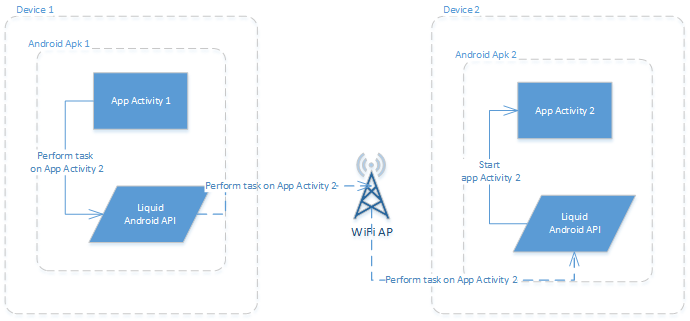
\includegraphics[width=.9\textwidth]{esempio2}
	\caption{Liquid Android API working example}
	\label{fig:3.4}
\end{figure}
In \figurename~\ref{fig:3.4} there is a scheme showing how the middleware could be used to build two different applications with two different packages (apk) including both the Liquid Android API which let them communicate by sending Android intent generated by \textit{Android Apk 1} and then received by \textit{Android Apk 2} installed respectively on two different devices.

\subsubsection{Data management} Last interesting scenario tu study is the data management problem in using such a system. This is a different type of scenario because it involves both previous scenarios. Having a distributed system always raises the problem of distributed data and data consistency. The middleware to be implemented must consider also the possibility to be used to build distributed Android applications in which data are generated somewhere by one device and then they need to be processed for a result by another one. A simple, but not trivial, example could be the case of a distributed calculator. A device acquires data and sends them to another one to be processed and then ask to that device the results. In the Android environment there is not the concept of distributed file system, so data involved in such an application must be considered and efficiently exchanged between devices.
\begin{figure}[h]
	\centering
	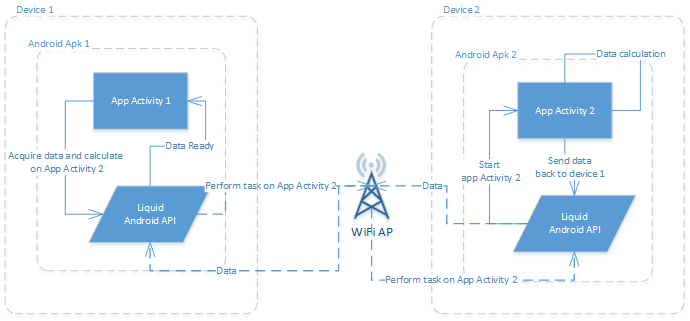
\includegraphics[width=.9\textwidth]{scenario3}
	\caption{Liquid Android API data management example}
	\label{fig:3.5}
\end{figure}

\section{Constraints} \label{problemconstraints}
In this section I would like to list a set of  constraints for the defined problem, that become requirements that the solution must meet. The section should be divided into two parts, the first for the requirements of the network, the second for the ones of the Android distributed intent generator and solver. The two sections are actually closely related so here I preferred to keep the two parts together, analyzing the entire middleware structure.\\ 
Here is the list:

\begin{itemize}
	\item \textit{M2M communication:} M2M communication is defined as a communication in which the two interlocutors are not humans. It is a communication completely handled by machines and computers \cite{cha2009trust}. It can be considered one of the fundamental enabling technologies of this thesis work, it permits object to communicate without humans being involved. In This type of communication the reader of the content is a computer, in this case are Android devices. The content of the messages must be well formed, the middleware must react properly to the event of receiving a distributed intent. So a clear, defined syntax with a well fixed structure  must be set in order to make everything understandable to a computer.
	
	\item \textit{Transparent:} As already widely discussed a middleware is those which do the \textit{magic}. The proposed solution is intended to be transparent to the Android OS and let it work as usual in resolving implicit intents whether they are distributed or not. Moreover as discussed in the chapter \ref{cap:statoarte}, to be more precise in \tablename~\ref{tab:transparency}, a distributed system must be transparent at many level, in this case the middleware must act as resources manager and efficiently mask resources access and location.
	
	
	\item \textit{Lightweight:} Another constraint to my system is the fact that whatever system I choose to be the solution it must be lightweight. This is needed because my system will work on a WiFi LAN. Messages must be encapsulated, serialized from one device and transferred in another one to be deserialized and analyzed to be executed. Messages must be as easy as they can because they are very frequent in such a system.
	
	\item \textit{Modular:} The implementation of the solution must be modular, this is due to the fact that this middleware is intended to be used as is but also to implement easily other kind of native Android distributed system application. Having a modular structure facilitates the specialization of its component and make all the middleware more readable and easy to use. In this way \text{Liquid Android} can be the substructure of other works.
	
	\item \textit{Extensible:} the implemented solution must meet canonical programming principles Extendability is one of the most important properties to take into account when building a computer system, especially when developing a middleware. Liquid Android modules have to be extensible to be improved or adapted to different purposes.
		
	\item \textit{Secure:} Liquid Android middleware must meet standard Android security design principles as described in \ref{androidsecurity}. The implementation must not exceed the limits imposed by the OS, I do not want to break the Android permission scheme and authorization model by \textit{rooting} the operating system, a process with which is possible to perform action as the administrator in Android environment. Rooting Android devices let application overcome the boundaries of standard applications, by letting them read and write data from all the OS. Moreover the middleware operates on mobile devices which usually contains and can manage many sensible and personal data, communications between these devices must be as secure as possible to limit security threats.
	
	\item \textit{Consistent:} Data and accessed resources involved in the system must meet consistency requirements. When developing distributed systems consistency is one of the main issue. The implemented solution must take into account data produced during the use of the system and make them consistent according to a chosen consistency model.
	
	\item \textit{Scalable:} the system to be implemented has not a fixed number of devices involved in. The chosen network architecture must be able to react according to the changes. Android devices are free to join or leave the network any time, and the system should be able to detect and maintain a dynamic network. Scalability is, in fact, the capability of a system, network, or process to handle a growing amount of work, or its potential to be enlarged in order to accommodate that growth \cite{bondi2000characteristics}. 
	
	\item \textit{Concurrent:} another important aspect of distributed systems is concurrency. Concurrency is the decomposability property of a program, algorithm, or problem into order-independent or partially-ordered components or units \cite{lamport1978time}. The implementation of the services must ensure this property to the system. The middleware has to have the capability to handle different requests at the same time and execute task in more than one device simultaneously.
	
\end{itemize}
The listed requirements, as already told in some of them, are, sometimes, general, in the sense that they have to be respected for the final product: a global and complete structure that starts from the construction of the network architecture arrives to the user's interaction activities on Android devices. This is because the problem I am facing is very big and complex, and it is transversal to the existing technologies, so the whole system must work properly. Keeping in mind what I have just stated, some of these constraints become fundamental requirements that my system must meet. My work has to be clear for developers to be used for further implementations of native Android distributed systems, but even if it can be less clear to an average user it must be usable to those wishing to try distributed intents with their own devices in a home LAN.

\bigskip
\bigskip
\bigskip
\bigskip
\bigskip
\bigskip
\par
In the next chapter I am presenting my idea, the \textit{Liquid Android} middleware, the so called solution to the given problem, explaining what I have done, my considerations about the situation here faced.

%
% -----------------------------END------------------------------------- %